\documentclass[cic,tc,english]{iiufrgs}
% Para usar o modelo, deve-se informar o programa e o tipo de documento.
% Programas :
% * cic       -- Graduação em Ciência da Computação
% * ecp       -- Graduação em Ciência da Computação
% * ppgc      -- Programa de Pós Graduação em Computação
% * pgmigro   -- Programa de Pós Graduação em Microeletrônica
% 
% Tipos de Documento:
% * tc                -- Trabalhos de Conclusão (apenas cic e ecp)
% * diss ou mestrado  -- Dissertações de Mestrado (ppgc e pgmicro)
% * tese ou doutorado -- Teses de Doutorado (ppgc e pgmicro)
% * ti                -- Trabalho Individual (ppgc e pgmicro)
% 
% Outras Opções:
% * english    -- para textos em inglês
% * openright  -- Força início de capítulos em páginas ímpares (padrão da
% biblioteca)
% * oneside    -- Desliga frente-e-verso
% * nominatalocal -- Lê os dados da nominata do arquivo nominatalocal.def


% Use unicode
\usepackage[utf8]{inputenc}   % pacote para acentuação
\usepackage[]{algorithm2e}


% Necessário para incluir figuras
\usepackage{graphicx}         % pacote para importar figuras

\usepackage{times}            % pacote para usar fonte Adobe Times
% \usepackage{palatino}
% \usepackage{mathptmx}       % p/ usar fonte Adobe Times nas fórmulas

\usepackage[alf,abnt-emphasize=bf]{abntex2cite}	% pacote para usar citações abnt

% 
% Informações gerais
% 
\title{A comparison of recommender systems for crowdfunding projects}

\author{Carniel Benin}{Adriano}
% alguns documentos podem ter varios autores:
% \author{Flaumann}{Frida Gutenberg}
% \author{Flaumann}{Klaus Gutenberg}

% orientador e co-orientador são opcionais (não diga isso pra eles :))
\advisor[Prof.~Dr.]{Castro da Silva}{Bruno}

% a data deve ser a da defesa; se nao especificada, são gerados
% mes e ano correntes
% \date{maio}{2001}

% o local de realização do trabalho pode ser especificado (ex. para TCs)
% com o comando \location:
\location{Porto Alegre}{RS}

% itens individuais da nominata podem ser redefinidos com os comandos
% abaixo:
% \renewcommand{\nominataReit}{Prof\textsuperscript{a}.~Wrana Maria Panizzi}
% \renewcommand{\nominataReitname}{Reitora}
% \renewcommand{\nominataPRE}{Prof.~Jos{\'e} Carlos Ferraz Hennemann}
% \renewcommand{\nominataPREname}{Pr{\'o}-Reitor de Ensino}
% \renewcommand{\nominataPRAPG}{Prof\textsuperscript{a}.~Joc{\'e}lia Grazia}
% \renewcommand{\nominataPRAPGname}{Pr{\'o}-Reitora Adjunta de P{\'o}s-Gradua{\c{c}}{\~a}o}
% \renewcommand{\nominataDir}{Prof.~Philippe Olivier Alexandre Navaux}
% \renewcommand{\nominataDirname}{Diretor do Instituto de Inform{\'a}tica}
% \renewcommand{\nominataCoord}{Prof.~Carlos Alberto Heuser}
% \renewcommand{\nominataCoordname}{Coordenador do PPGC}
% \renewcommand{\nominataBibchefe}{Beatriz Regina Bastos Haro}
% \renewcommand{\nominataBibchefename}{Bibliotec{\'a}ria-chefe do Instituto de Inform{\'a}tica}
% \renewcommand{\nominataChefeINA}{Prof.~Jos{\'e} Valdeni de Lima}
% \renewcommand{\nominataChefeINAname}{Chefe do \deptINA}
% \renewcommand{\nominataChefeINT}{Prof.~Leila Ribeiro}
% \renewcommand{\nominataChefeINTname}{Chefe do \deptINT}

% A seguir são apresentados comandos específicos para alguns
% tipos de documentos.

% Relatório de Pesquisa [rp]:
% \rp{123}             % numero do rp
% \financ{CNPq, CAPES} % orgaos financiadores

% Trabalho Individual [ti]:
% \ti{123}     % numero do TI
% \ti[II]{456} % no caso de ser o segundo TI

% Monografias de Especialização [espec]:
% \espec{Redes e Sistemas Distribuídos}      % nome do curso
% \coord[Profa.~Dra.]{Weber}{Taisy da Silva} % coordenador do curso
% \dept{INA}                                 % departamento relacionado

% 
% palavras-chave
% iniciar todas com letras minúsculas, exceto no caso de abreviaturas
% 
\keyword{UFRGS}
\keyword{recommender systems}
\keyword{AI}
\keyword{crowdfunding}

%\settowidth{\seclen}{1.10~}

% 
% inicio do documento
% 
\begin{document}

% folha de rosto
% às vezes é necessário redefinir algum comando logo antes de produzir
% a folha de rosto:
% \renewcommand{\coordname}{Coordenadora do Curso}
\maketitle

% dedicatoria
% \clearpage
% \begin{flushright}
%     \mbox{}\vfill
%     {\sffamily\itshape
%       ``If I have seen farther than others,\\
%       it is because I stood on the shoulders of giants.''\\}
%     --- \textsc{Sir~Isaac Newton}
% \end{flushright}

% agradecimentos
%\chapter*{Agradecimentos}
%Agradeço ao \LaTeX\ por não ter vírus de macro\ldots



% resumo na língua do documento
\begin{abstract}
    Este documento é um exemplo de como formatar documentos para o
    Instituto de Informática da UFRGS usando as classes \LaTeX\
    disponibilizadas pelo UTUG\@. Ao mesmo tempo, pode servir de consulta
    para comandos mais genéricos. \emph{O texto do resumo não deve
      conter mais do que 500 palavras.}
\end{abstract}

% resumo na outra língua
% como parametros devem ser passados o titulo e as palavras-chave
% na outra língua, separadas por vírgulas
\begin{englishabstract}{Using \LaTeX\ to Prepare Documents at II/UFRGS}{Electronic document preparation. \LaTeX. ABNT. UFRGS}
    This document is an example on how to prepare documents at II/UFRGS
    using the \LaTeX\ classes provided by the UTUG\@. At the same time, it
    may serve as a guide for general-purpose commands. \emph{The text in
      the abstract should not contain more than 500~words.}
\end{englishabstract}

% lista de figuras
\listoffigures

% lista de tabelas
\listoftables

% lista de abreviaturas e siglas
% o parametro deve ser a abreviatura mais longa
\begin{listofabbrv}{SPMD}
    \item[SMP] Symmetric Multi-Processor
    \item[CBF] Content-based filtering
    \item[CF] Collaborative filtering
    \item[SPMD] Single Program Multiple Data
    \item[ABNT] Associação Brasileira de Normas Técnicas
\end{listofabbrv}

% idem para a lista de símbolos
% \begin{listofsymbols}{$\alpha\beta\pi\omega$}
%     \item[$\sum{\frac{a}{b}}$] Somatório do produtório
%     \item[$\alpha\beta\pi\omega$] Fator de inconstância do resultado
% \end{listofsymbols}

% sumario
\tableofcontents

% aqui comeca o texto propriamente dito

% introducao
\chapter{Introdução}
No início dos tempos, Donald E. Knuth criou o \TeX. Algum tempo depois, Leslie Lamport criou o \LaTeX. Graças a eles, não somos obrigados a usar o Word nem o LibreOffice.

%% \section{Figuras e tabelas}

%% Esta seção faz referência às Figuras~\ref{fig:estrutura},~\ref{fig:ex1} e~\ref{fig:ex2}, a título de exemplo. A primeira figura apresenta a estrutura de uma figura. A \emph{descrição} deve aparecer \textbf{acima} da figura. Abaixo da figura, deve ser indicado a origem da imagem, mesmo se essa for apenas os autores do texto.

%% A Figura~\ref{fig:ex1} representa o caso mais comum, onde a figura propriamente dita é importada de um arquivo ( neste exemplo o formato é \texttt{eps} ou \texttt{pdf}. Veja a seção \ref{sec:fig_format}). A Figura~\ref{fig:ex2} exemplifica o uso do environment \texttt{picture}, para desenhar usando o próprio~\LaTeX.

%% \begin{figure}[h]
%%     \caption{Descrição da Figura deve ir no topo}
%%     \begin{center}
%%         % Aqui vai um includegraphics , um picture environment ou qualquer
%%         % outro comando necessário para incorporar o formato de imagem
%%         % utilizado.        
%%         \begin{picture}(100,100)
%%             \put(0,0){\line(0,1){100}}
%%             \put(0,0){\line(1,0){100}}
%%             \put(100,100){\line(0,-1){100}}
%%             \put(100,100){\line(-1,0){100}}
%%             \put(10,50){Uma Imagem}
%%         \end{picture}    
%%     \end{center}
%%     \label{fig:estrutura}
%%     \legend{Fonte: Os Autores}
%% \end{figure}

%% \begin{figure}
%%     \caption{Exemplo de figura importada de um arquivo e também exemplo de caption muito grande que ocupa mais de uma linha na Lista~de~Figuras}
%%     \begin{center}
%%         \includegraphics[width=8em]{fig}
%%     \end{center}
%%     \legend{Fonte: Os Autores}
%%     \label{fig:ex1}
%% \end{figure}

% o `[h]' abaixo é um parâmetro opcional que sugere que o LaTeX coloque a
% figura exatamente neste ponto do texto. Somente preocupe-se com esse tipo
% de formatação quando o texto estiver completamente pronto (uma frase a mais
% pode fazer o LaTeX mudar completamente de idéia sobre onde colocar as
% figuras e tabelas)
% \begin{figure}[h]
%% \begin{figure}
%%     \caption{Exemplo de figura desenhada com o environment \texttt{picture}.}
%%     \begin{center}
%%         \setlength{\unitlength}{.1em}
%%         \begin{picture}(100,100)
%%             \put(20,20){\circle{20}}
%%             \put(20,20){\small\makebox(0,0){a}}
%%             \put(80,80){\circle{20}}
%%             \put(80,80){\small\makebox(0,0){b}}
%%             \put(28,28){\vector(1,1){44}}
%%         \end{picture}
%%     \end{center}
%%     \legend{Fonte: Os Autores}
%%     \label{fig:ex2}
%% \end{figure}

%% Tabelas são construídas com praticamente os mesmos comandos. Ver a tabela \ref{tbl:ex1}.

%% \begin{table}[h]
%%     \caption{Uma tabela de Exemplo}
%%     % OBS: não use \begin{center}, pois este aumenta o espaçamento entre a caption/legend e a tabela
%%     % Para figuras, a aparência é melhor com o espaçamento extra
%%     \centering
%%         \begin{tabular}{c|c|p{5cm}}
%%           \hline
%%           \textit{Col 1}  &   \textit{Col 2}  &   \textit{Col 3} \\
%%           \hline
%%           \hline
%%           Val 1           &   Val 2           & Esta coluna funciona como um parágrafo, tendo uma margem definida em 5cm. Quebras de linha funcionam como em qualquer parágrafo do tex. \\
%%           Valor Longo     & Val 2             & Val 3 \\
%%           \hline
%%         \end{tabular}
%%     \legend{Fonte: Os Autores}
%%     \label{tbl:ex1}
%% \end{table}

%% \subsection{Formato de Figuras}
%% \label{sec:fig_format}

%% O LaTeX permite utilizar vários formatos de figuras, entre eles \emph{eps}, \emph{pdf}, \emph{jpeg} e \emph{png}. Programas de diagramação como Inkscape (e mesmo LibreOffice) permitem gerar arquivos de imagens vetoriais que podem ser utilizados pelo LaTeX sem dificuldade. Pacotes externos permitem utilizar SVG e outros formatos.

%% Dia e xfig são programas utilizados por dinossauros para gerar figuras vetoriais. Se possível, evite-os.

%% \subsection{Classificação dos etc.}

%% O formato do instituo de informática define 5 níveis: capítulo, seção, subseção e outros 2 sem nome.

%% \subsubsection{Subsubseção}
%% Exemplo de uma subsubseção.

%% \paragraph{Parágrafo}
%% Exemplo de um parágrafo.

%% \section{Sobre as referências bibliográficas}

%% A classe \emph{iiufrgs} faz uso do pacote \emph{abnTeX2} com algumas alterações
%% feitas por Sandro Rama Fiorini. Culpe ele se algo der errado. Agradeça a ele
%% pelo que der certo. As modificações dão uma camada de tinta NATBIB-style,
%% já que o abntex2 usa uns comandos de citação feitos para alienígenas de 5 braços
%% wtf. Exemplos de citação:

%% \begin{itemize}
%%     \item \emph{cite}: Unicórnios são verdes \cite{Adams2009Conceptual};
%%     \item \emph{citep}:Unicórnios são verdes \citep{Adams2009Conceptual};
%%     \item \emph{citet}: Segundo \citet{Adams2009Conceptual}, unicórnios são
%%     verdes.
%%     \item \emph{citen or citenum}: Segundo \citen{Adams2009Conceptual},
%%     unicórnios são verdes.
%%     \item \emph{citeauthor e citeyearpar}: Segundo artigos de
%%     \citeauthor{Adams2009Conceptual} , unicórnios são azuis
%%     \citeyearpar{Adams2009Conceptual}.

%% \end{itemize}

%% O estilo abnt fornecido antigamente pelo UTUG não é mais recomendado, pois não
%% produz saída de acordo com as exigências da biblioteca.

%% Recomenda-se o uso de bibtex para gerenciar as referências (veja o arquivo
%% biblio.bib).

% e aqui vai a parte principal
\chapter{Recommendation Algorithms}
Recommendation Algorithms are widely used in the industry today to provide useful suggestions to end-users in a completely automated manner. They are ubiquitous in modern e-commerce Web sites \cite{Schafer2001}, where new products can be recommended based on a customer's interests and preferences, and in many other fields such as movies (Netflix) and music (Spotify). Its importance can't be overstated: the effectiveness of targeted recommendations, as measured by click-through and conversion rates, far exceed those of untargeted content \cite{Linden2003}.

The basic idea behind any recommender system is to obtain a utility function to estimate a user preferences towards an item. The meaning of this function will differ for each context; it could mean how likely a user will want to watch a specific movie or listen to a song, or the likelihood of buying a particular product. In our case, the goal is to find projects the customer is most likely to back given his backing history and other characteristics. 

Recommender systems can be broadly divided into two categories: content-based methods and collaborative filtering methods \cite{Rakesh2016}.
The former utilizes the content features of users or items in order to recommend items to users. In collaborative filtering methods, user ratings and other data are used in order to calculate similarities between users or items, which are then ranked to show the most relevant recommendations. These two methods are sometimes combined into what is known as Hybrid Recommender Systems.
\section{Collaborative filtering}
Collaborative filtering is based on the principle that similar users will share similar interests. In the traditional approach, each customer is represented by a \(N\)-dimensional vector of items, where \(N\) stands for the number of available items, and each vector component corresponds to the user rating of the item. These ratings can be obtained explicitly - e.g. star rating or "likes" - or implicitly - e.g. a user buying an item or listening to a song can be considered a positive rating. By collecting ratings from each user, we build a \(R_{nxm}\) matrix which is the starting point for CF. For most applications, \(R\) will be extremely sparse, our job then is to try to predict the missing ratings.

CF algorithms can be further divided into Memory-Based and Model-Based techniques. Memory-Based algorithms use a dataset of user-item pairs to identify groups of similar users, which are in turn used to make predictions of preference for new items. In Model-Based methods, machine learning algorithms are used to develop a model that will be used to predict user ratings. These methods can solve some of the shortcomings of Memory-Based approaches, such as the need for large rating matrices. Finally, both approaches can be combined into Hybrid Recommenders. A overview of these techniques is depicted in ~\ref{fig:cf-comparison}.

For large databases, CF can be prohibitively computationally expensive. Its worst case performance is \(O(MN)\) where \(M\) is the number of customers and \(N\) is the number of items \cite{Linden2003}, but this problem can be generally alleviated due to the customer vector sparsity. Item-to-item CF is another method proposed by Amazon that tries to minimize these scaling issues by focusing on item instead of user similarity. Each item purchased by the customer is compared to other items in the dataset in order to calculate a similarity metric. The algorithm is shown bellow:

\begin{algorithm}[H]
 \For{each item in product catalog, I1}{
  \For{each customer C who purchased I1}{
    \For{item I2 purchased by customer C}{
      Record that a customer purchased I1 and I2\;
    }
  }
  \For{each item I2}{
    Compute the similarity between I1 and I2\;
  }
 }
 \caption{Item-to-item CF}
\end{algorithm}

There are many ways to compute the similarity between items, one common method is the cosine measure defined as follows:

\(similarity(\pmb x, \pmb y) = cos(\pmb x, \pmb y) = \frac {\pmb x \cdot \pmb y}{||\pmb x|| \cdot ||\pmb y||}\)


In either case, for this to work large amounts of user data is required. This is known as the cold start problem: new users who haven't rated many items yet will have a reduced recommendation quality. On the other hand, no information about the item itself is needed, making CF specially applicable to collections of hard-to-analyze items such as movies.

\begin{figure}
    \caption{Overview of collaborative filtering techniques.}
    \begin{center}
        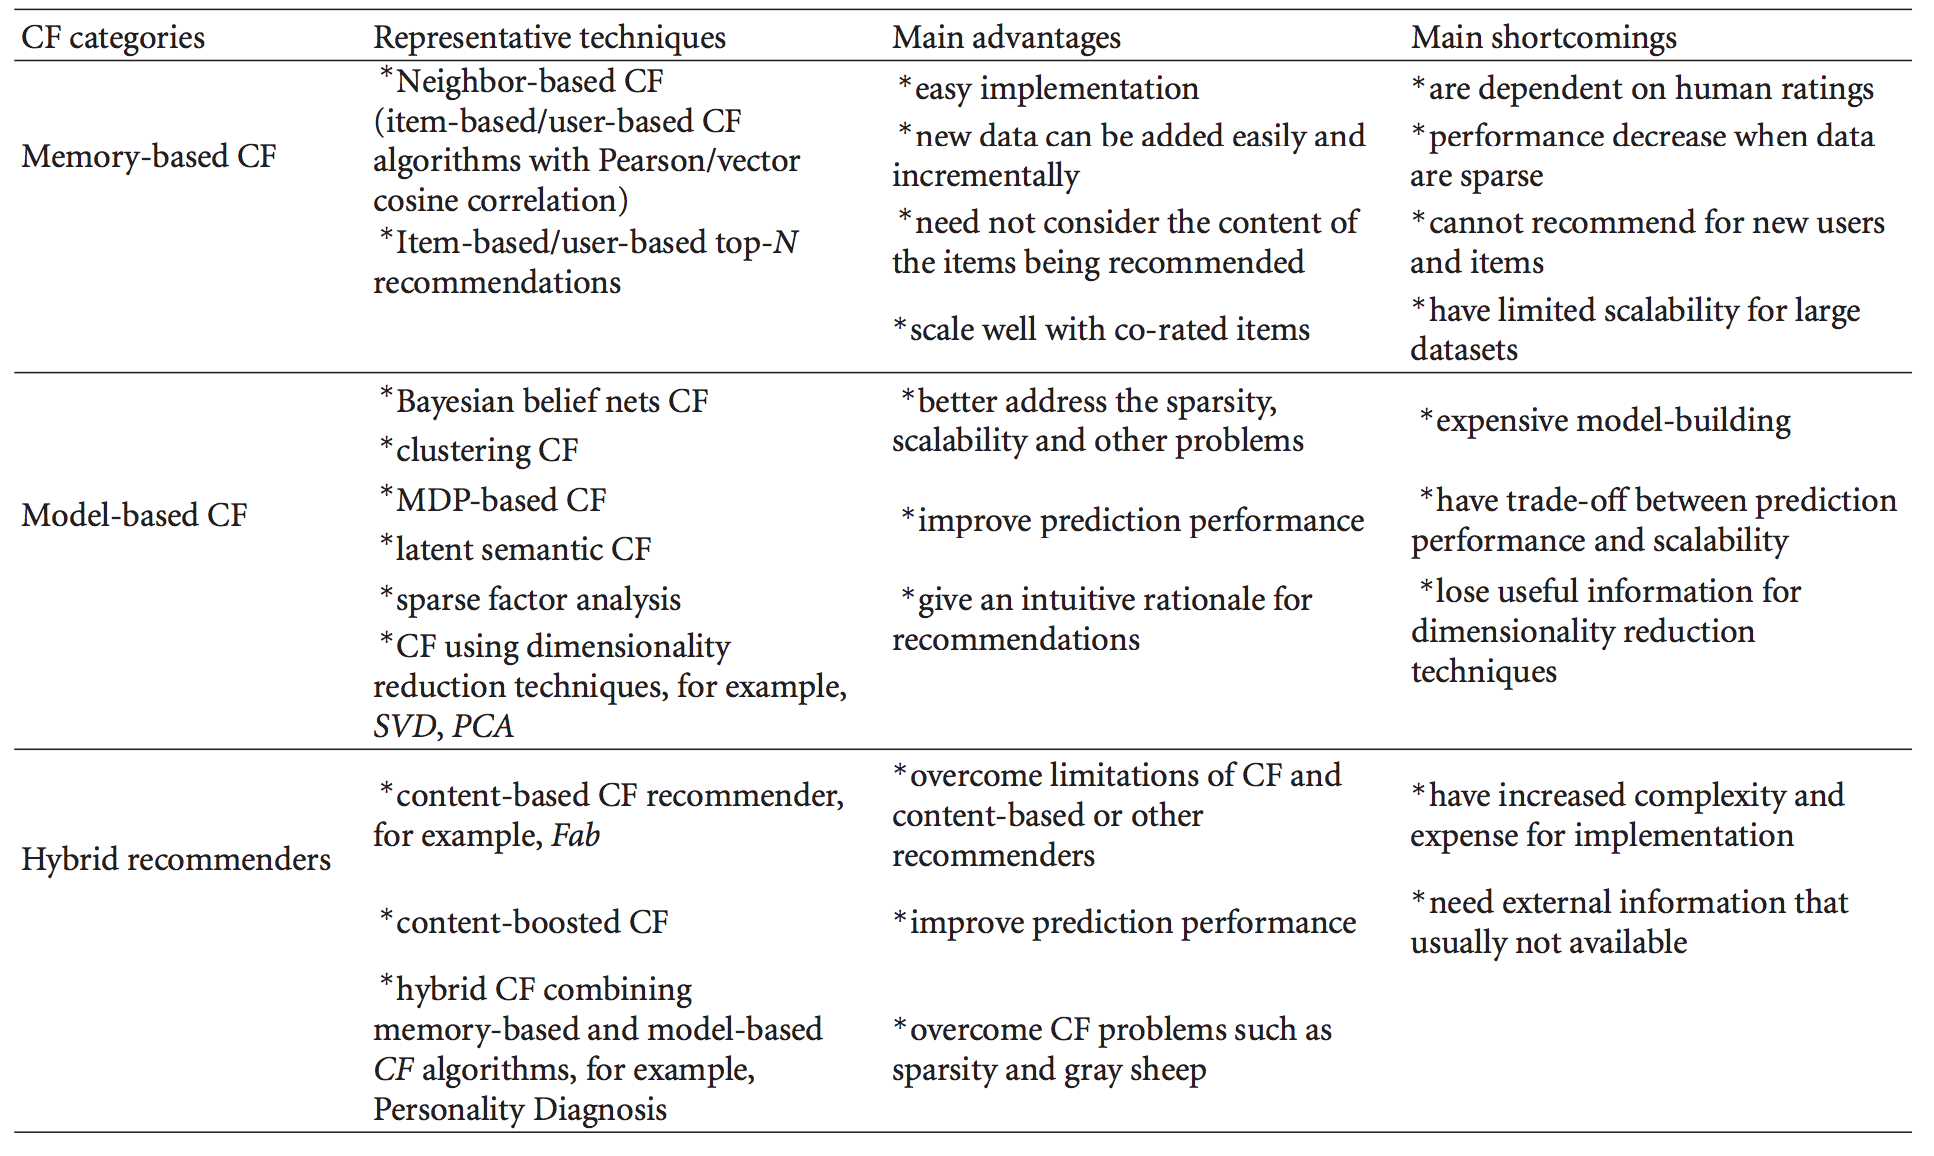
\includegraphics[width=35em]{cf-comparison}
    \end{center}
    \label{fig:cf-comparison}
    \legend{Source: \cite{Su2009}}
\end{figure}

\section{Content-based filtering}
In this method a description of each item is constructed using structured data or some sort of item presentation algorithm such as Latent Dirichlet Allocation or TF-IDF. This representation is then compared to the user profile and the best-matching items are recommended. The user profile can consist of many different types of information: a history of the user's interaction with the system such as page views, searches and purchases is often used to train the model without any explicit user input. Some systems may require the user to explicitly state his interests, however it may be very hard to get users to make this effort, rendering this approach very limited in practice.

As CBF focus on item rather than user similarity, it avoids the cold start problem since little information about user preference is needed. However, since only similar items to those already rated by the user will be considered, CBF approaches tend to suffer from over-specialization \cite{Iaquinta2008}. This is known as the serendipity problem. Another limitation of CBF algorithms is that items are required to contain enough information in order to distinguish items the user likes from items the user doesn't like. For example, a dataset of songs where only the song name is available would not be enough to make good predictions based on this content only, however this would pose no problem for collaborative filtering methods which rely solely on user similarity. 




\chapter{About Catarse}
Launched in January 2011, Catarse was the first crowdfunding platform for creative projects in Brazil. With over 7000 successfully financed projects raising R\$77 millions from 480.000 people, it's currently the largest national platform of its kind. It works similarly to most crowdfunding platforms: the project owner presents his or her idea and specifies the required investment as well as the cutoff date for the project, while offering rewards for those who back it. Projects are divided into 3 main categories: all-or-nothing, flexible and recurrent. In the first type, projects are available for backing up to 60 days and the project owner only receives the raised amount if the project's goal is met, otherwise all the money is returned to its original backers. On flexible projects the owner receives the raised amount whether the goal is reached or not. Recurrent projects are subscription based and the owner can collect the money monthly. This work will only focus on the first two types of projects.

\chapter{Recommending projects}
Catarse's dataset is unique in a variety of ways that makes collaborative filtering techniques hard to apply. Firstly, unlike regular e-commerce Web sites such as Amazon where products stay available for many years, crowdfunding projects have a predetermined cutoff date, after which it's no longer possible to make a pledge. It makes no sense to recommend expired projects, severely limiting our training data to online projects only. Another challenge is the fact that the majority of Catarse's users only back one project, making it very hard to get enough data for CF methods to work properly. Our only choice is then to use content-based methods, this allows us to train our model with the whole dataset to extract backer-project features, and later use this model to search for online projects with the highest backing probability for the current user.

\section{Data preparation}
The dataset \(D\) was obtained directly from Catarse's production database. Each training example consists of a project-backer pair \((p,b)\) with 12 dimensions presented below:
\begin{itemize}

    \item \emph{category count}: Number of projects backed by the user \(b\) in the same category as project \(p\)
    \item \emph{mode count}: Number of projects backed by the user \(b\) with the same mode (aon, flex or sub) as project \(p\)
    \item \emph{same state}: True if the project location is the same as the backer's
    \item \emph{recommended}: True if project \(p\) was manually recommended by an admin
    \item \emph{has video}: True if the project has uploaded a video
    \item \emph{budget}: Budget text length in chars
    \item \emph{description}: Description text length in chars
    \item \emph{pledged}: Amount pledged in the first 3 days
    \item \emph{contributions}: Amount of contributions in the first 3 days
    \item \emph{progress}: Percentage of goal reached in the first 3 days
    \item \emph{owner projects}: Amount of projects from the same project owner as \(p\)
    \item \emph{reward count}: Number of offered rewards in project \(p\)
\end{itemize}

In order to trim irrelevant data, we remove canceled and draft projects as well as projects with no backers from the dataset. The final cardinality of \(D\) was 300000. For the sake of balancing our dataset, we create 300000 more negative instances by randomly combining users with projects they haven't backed. To further emphasize project quality, only successful projects are considered for the positive instances, while only failed projects are used for the negative instances. Finally, due to changes in the platform that occurred in 2015, we ignore data from earlier periods so as to maintain a consistent dataset.

\begin{figure}
    \caption{Feature weights in gbtree}
    \begin{center}
        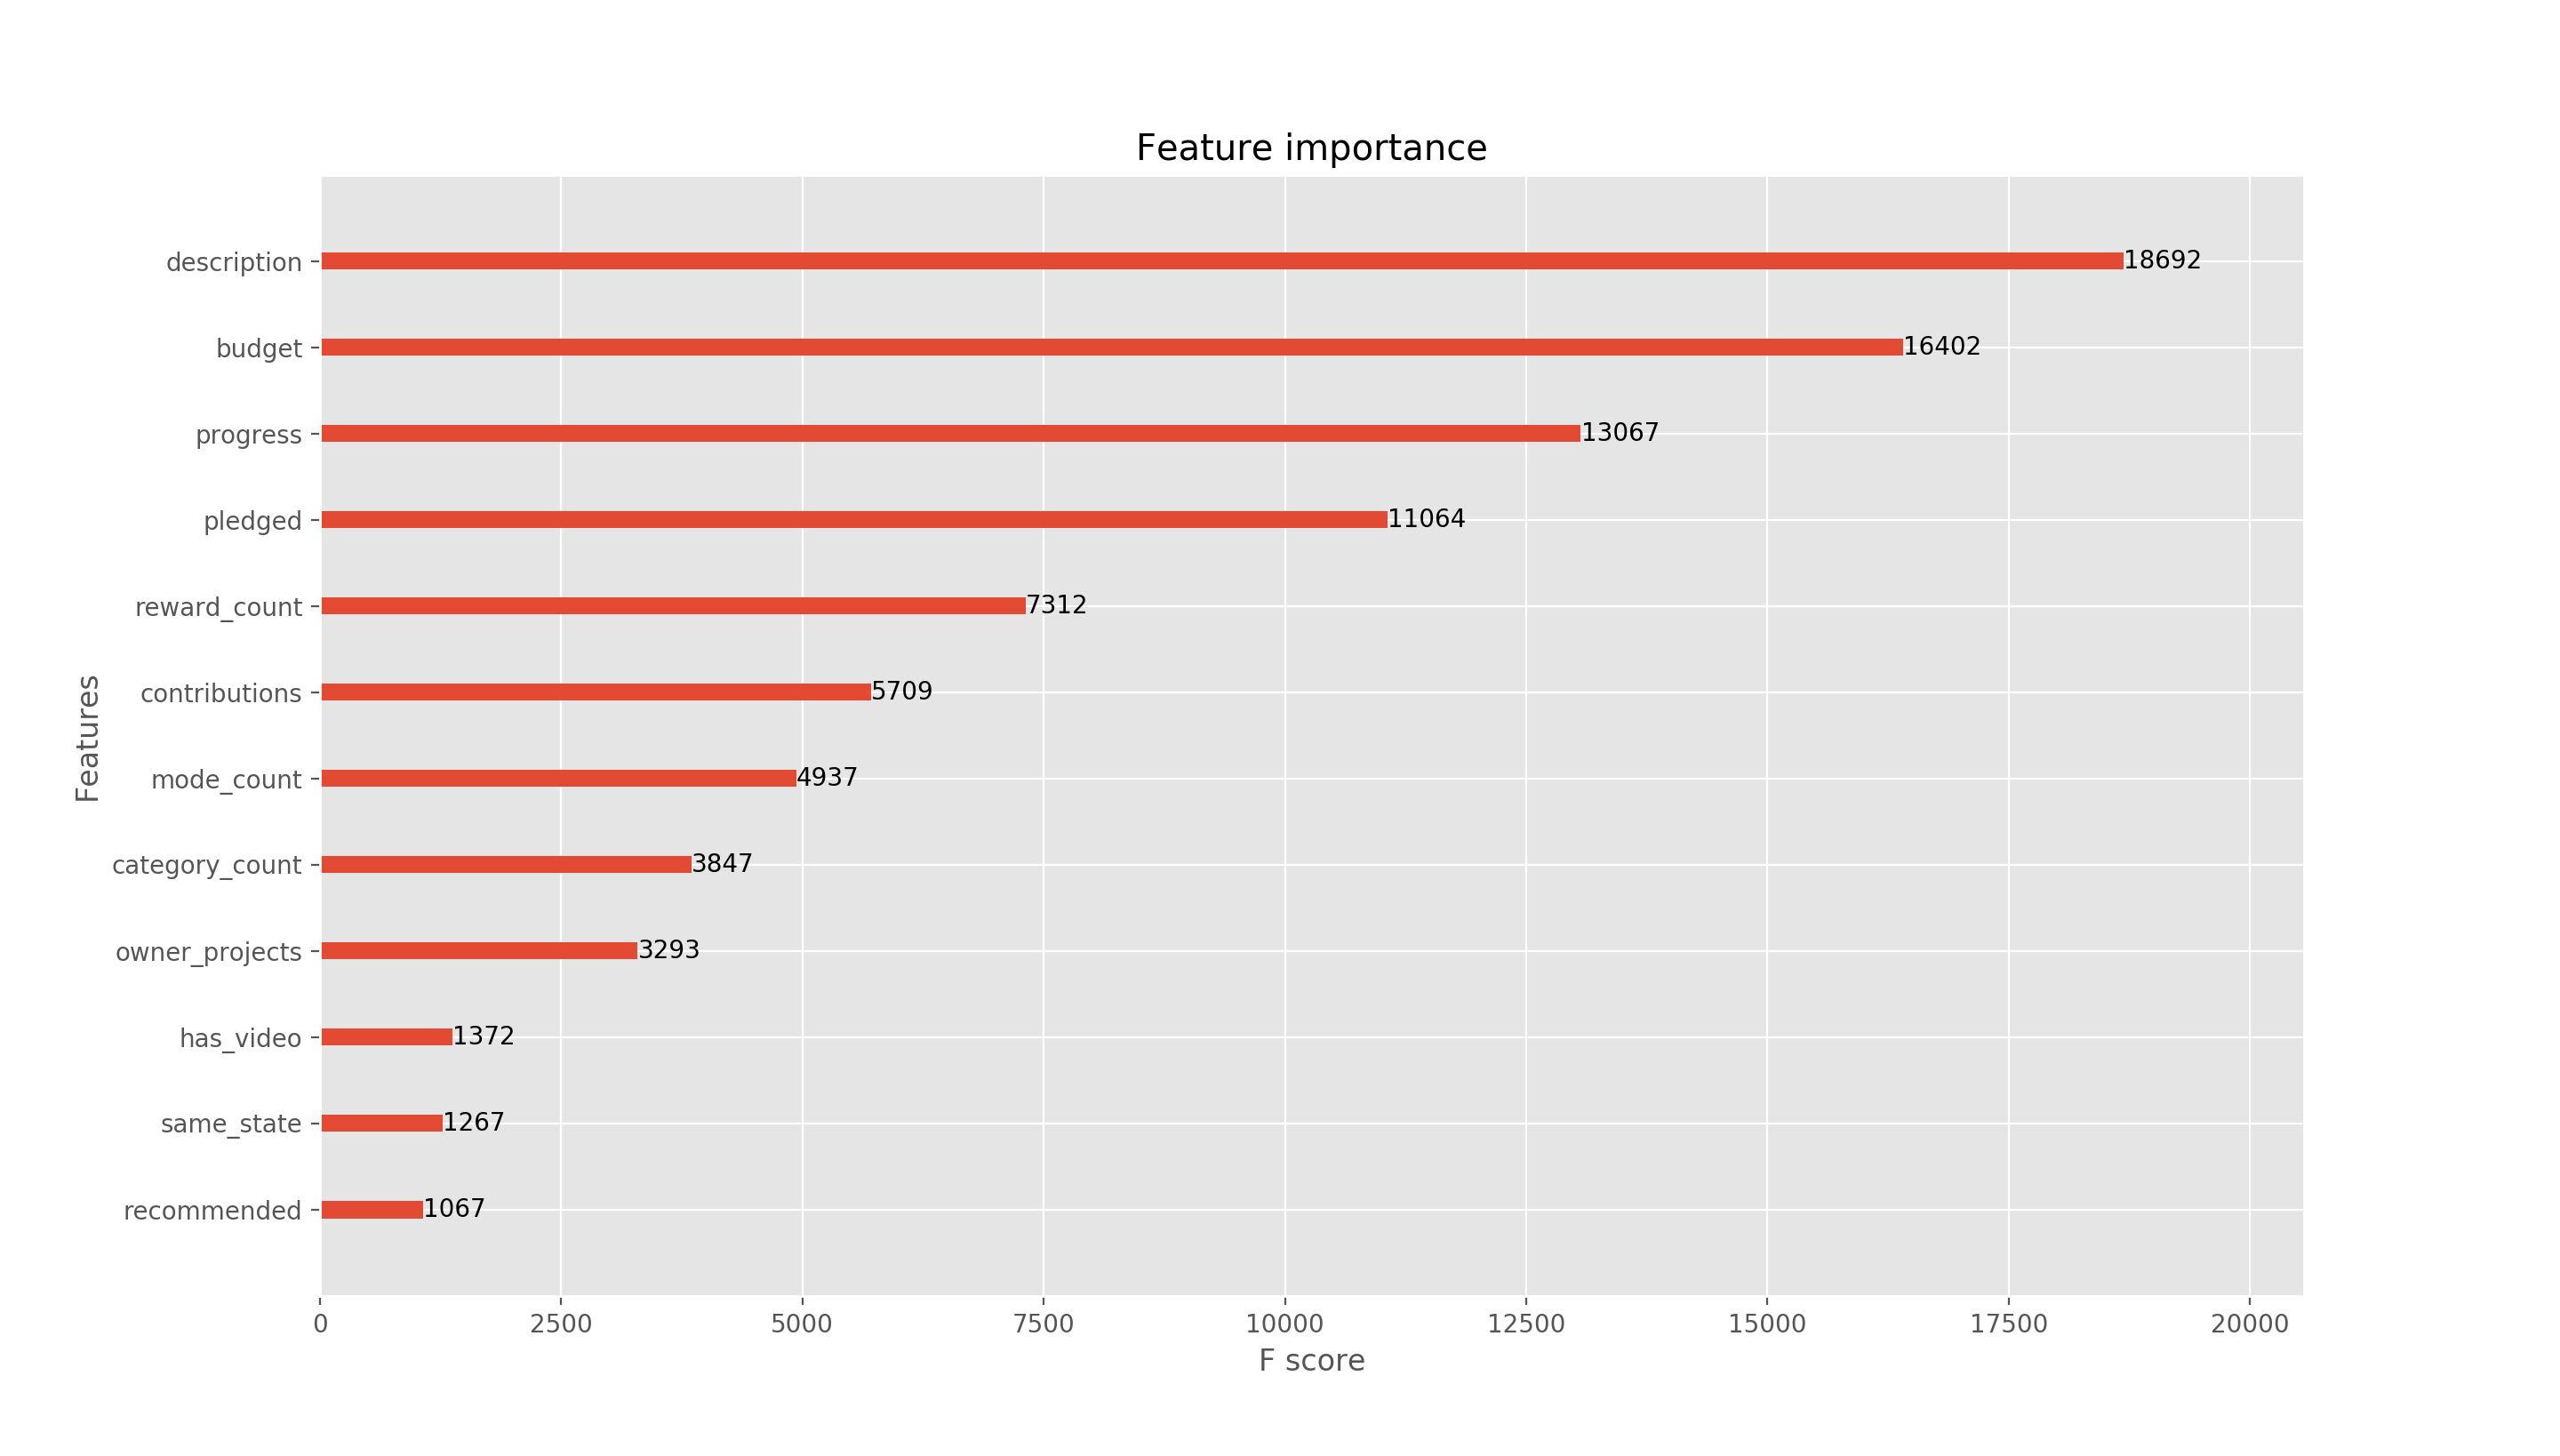
\includegraphics[width=35em]{featureweights}
    \end{center}
    \label{fig:features}
\end{figure}

\chapter{Gradient boosting trees}
In recent years, tree boosting has become a increasingly popular method and been shown to give state-of-the-art results for many classification problems \cite{Li2012}. As in any supervised learning method, our objective is to train a model to predict a target variable \(y_i\) given features \(x_i\). Boosting methods are characterized by combining many weak learners into a strong one in a iterative fashion. In this case, our model is an ensemble of trees, more specifically a set of classification and regression trees (CART). Unlike decision trees, where the leafs contain decision values, the leafs on gradient boosting trees contain a score \(s \in \mathbb{R}\). Multiple simple trees are then constructed and the prediction of each tree is summed up to get the final score ~\ref{fig:ex1}. Our model can then be defined as

\(\hat{y}_i = \sum_{k=1}^K f_k(x_i), f_k \in \mathcal{F}\)

where \(K\) is the number of trees, \(f\) is a function in the functional space \mathcal{F}, and \mathcal{F} is the set of all possible CARTs \cite{Chen2016}. Our objective function can the be written as

\(\text{obj}(\theta) = \sum_i^n l(y_i, \hat{y}_i) + \sum_{k=1}^K \Omega(f_k)\)

\begin{figure}
    \caption{GbTree example}
    \begin{center}
        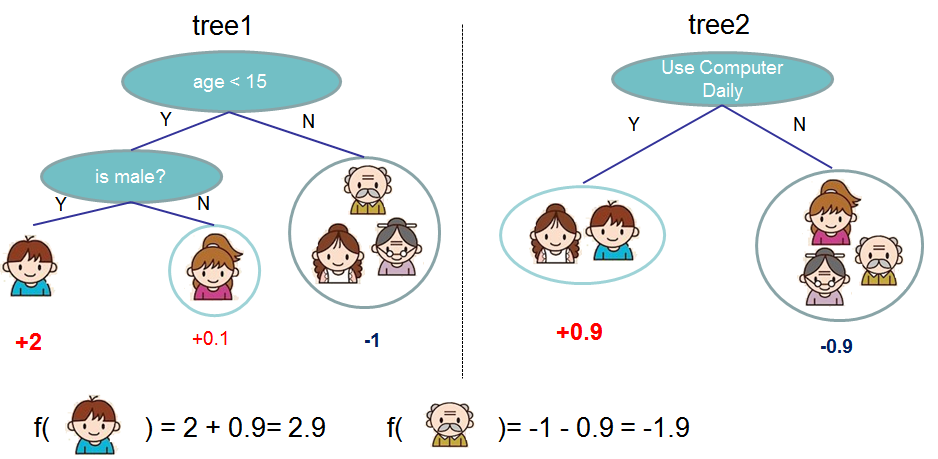
\includegraphics[width=28em]{twocart}
    \end{center}
    \legend{Source: XGBoost official site}
    \label{fig:ex1}
\end{figure}

\section{Objective function}
Our objective function is used to measure the performance of our model for each set of parameters. We define it as the sum of the training loss function \(L\) with the regularization term \Omega.

\(\text{obj}(\theta) = L(\theta) + \Omega(\theta)\)

In this work we define our loss function as the logistic loss function for logistic regression.

\(L(\theta) = \sum_i[ y_i\ln (1+e^{-\hat{y}_i}) + (1-y_i)\ln (1+e^{\hat{y}_i})]\)

And our regularization function is defined as follows:

\(\Omega(f) = \gamma T + \frac{1}{2}\lambda \sum_{j=1}^T w_j^2\)

Where \(w\) is the vector of scores on leaves and \(T\) is the number of leaves.

After defining our objective function, we optimize it in order to train our model.

\chapter{Implementation}
The XGBoost python library was used to create our gradient boosting tree model. Hyperparameters were tuned by running 10-fold cross validation while optimizing for negative log-likelihood. No data standardization or normalization was necessary since the base learners are trees.


% \chapter{Estado da arte}
% \chapter{Mais estado da arte}
% \chapter{A minha contribuição}
% \chapter{Prova de que a minha contribuição é válida}
% \chapter{Conclusão}

% referências
% aqui será usado o environment padrao `thebibliography'; porém, sugere-se
% seriamente o uso de BibTeX e do estilo abnt.bst (veja na página do
% UTUG)
% 
% observe também o estilo meio estranho de alguns labels; isso é
% devido ao uso do pacote `natbib', que permite fazer citações de
% autores, ano, e diversas combinações desses

\bibliographystyle{abntex2-alf}
\bibliography{cic-tc}{}

\end{document}
